\chapter{Palabras acumuladas}

La búsqueda para cuantificar la influencia que tiene un idioma, ha llevado a contabilizar las palabras que son nuevas en los distintos receptores y a partir de ellas ligar contextos que amplíen la forma de influencia.  Se ha puesto también énfasis en el conjunto de búsqueda, pero  el conjunto base  también tiene información de cuáles palabras han migrado, además  abarca más años (160 entre 1740 y 2009), por lo que su información es más basta en contenido. 

Para no repetir el proceso de contabilizar a los préstamos nuevos,  se propone pensar que en el primer año del conjunto de búsqueda (1900),  el idioma receptor ya contenía cierta cantidad de palabras que provenían de otros orígenes,  de tal manera que ya forman parte de él, es decir estos préstamos “conviven” con las palabras propias del receptor. Es necesario hacer una nueva definición para estos préstamos.   Dados un idioma  origen  \textit{A} y  la lista para un año  de las palabras más comunes en el receptor \textit{B},  se detonan como: 

\begin{description}
	\item[Préstamos acumulados:] Son las palabras con origen \textit{A} que ya habían aparecido en alguna lista de \textit{B}, y para ese año lo volvieron a hacer.  
\end{description}

La diferencia entre los nuevos y los acumulados es que sólo serán nuevos en el primer año de aparición,  posteriormente a él se convierten en acumulados. 


El objetivo de este estudio es ver cómo se comportan todas las palabras que ya han migrado a un receptor, y si hay una tendencia donde su uso sea alterado. 

Continuando con las distinciones, el método del capitulo anterior se enfoca en la cantidad de palabras nuevas, nunca se trato con la frecuencia de las palabras, ahora se utilizará esta propiedad  para llegar a una cuantificación de la influencia. Si se tienen la lista de las cinco mil palabras más usadas  de \textit{B}, y se distinguen aquellas que provienen de un origen \textit{A} que han aparecido con anterioridad, es decir los préstamos acumulados de \textit{A} en \textit{B}, entonces el proceso para cuantificar el uso de \textit{A} en \textit{B} es el siguiente: 

\newpage

\begin{enumerate}
	
	\item En un año determinado del idioma \textit{B}, se sumarán las frecuencias $f_{i}$ de las cinco mil palabras más usadas.  Esta cantidad se llamará \textbf{frecuencia total por año.}
	
	\begin{equation}
	\label{ec.ftot}
	f_{t} = \sum_{i=1}^{5000} f_{i} \,\,\,\,\,\,\,\,\, i = posici\acute{o}n\,\, de \,\,cada \,\,palabra
	\end{equation}
	
	\item Como se conocen las posiciones $j$,  que ocupan los préstamos \textit{A} en la lista de \textit{B}, se procede a sumar sólo las frecuencias asociadas a estas palabras. Esta cantidad será la \textbf{frecuencia de préstamo} $f_{p}$,  siempre será menor que la frecuencia total por año.
	
	\begin{equation}
	\label{ec.fpres}
	f_{p} = \sum_{j} f_{j} \,\,\,\,\,\,\,\,\, j = posici\acute{o}n\,\, de \,\,cada \,\,pr\acute{e}stamo
	\end{equation}
	
	
	\item  Se divide la frecuencia de préstamo entre la frecuencia total por año, esta cantidad se llamará  \textbf{Uso} $U$ y es la porción que representa \textit{A} en \textit{B} en teŕminos de frecuencia, \textit{El uso de A en B}.  Como en un año hay mas palabras propias de B, esta cantidad es muy pequeña, para tener cifras manejables, se tomara un porcentaje al multiplicar el cociente por cien, así la frecuencia de uso es siempre positiva y toma valores entre cero y cien.  

	\begin{equation}
	\label{ec.fuso}
	 U = \frac{f_{p}}{f_{t}} * 100
	\end{equation}
	
	
	Entre más cercana a 100$\%$ sea el \textit{Uso de A en B}, los préstamos de \textit{A} son más relevantes en \textit{B}.

\end{enumerate}

Entonces,  la nueva forma de medir influencia sera mediante el uso. Lo relevante de trabajar con este método es que  en un determinado año o conjunto de años, se puede ver el uso que han tenido los prestamos con diferentes orígenes en un mismo receptor ó el proceso inverso,  observando el uso que ha tenido un origen en los diferentes receptores. 




\newpage

\section{La influencia en 109 años}

Descritas el tipo de palabras a emplear y la forma de trabajar con ellas, el proceso que se siguió para obtener resultados es el siguiente: 

\begin{itemize}
	
	\item Elegidos un  origen \textit{A} y un receptor \textit{B}, se localizaron en el conjunto base los prestamos acumulados de \textit{A} en \textit{B}. Obteniendo una base de las palabras que ya forman parte de \textit{B} al comienzo del conjunto de búsqueda. 
	
	\item Se empleó la ecuación \ref{ec.fuso} en todos los años del conjunto de búsqueda, obteniendo 109 valores.
	
	\item El proceso se repitió para todas las combinaciones de orígenes y receptores.
	
	\item  Tras cada año del conjunto de búsqueda, se elaboraron nuevas listas de los prestamos acumulados, agrupándolos por cada combinación de origen y receptor. 
	
	\item Para observar los datos como una cantidad que varia en el tiempo, se  hicieron tres tipos de graficas con tres tipos de agrupaciones.
	
	\begin{description}
		
		\item[\textit{A} como origen común.] Graficando el uso de \textit{A} en todos los demás idiomas para observar en que idiomas \textit{A} es más empleado. 
		
		\item[\textit{A} como receptor común.] Graficando el uso de los demás en \textit{A}, observando que idioma es mas empleado en \textit{A}.
		
		\item[Alternando \textit{A} y \textit{B}.]  Se graficó de manera conjunta el uso de \textit{A} en \textit{B}, y el de \textit{B} en \textit{A}, observando en cuales momentos uno fue mas empleado que el otro.
		
		%\item Como se esta trabajando en un periodo de ciento nueve años, el uso será mayor o menor en determinadas épocas; para no repetir el proceso anterior de dividir por décadas, se especificara el periodo donde se tuvo el mayor cambio en el uso y los años que se abarcaron.  
		 
		
	\end{description}	

\end{itemize}

Las listas elaboradas se emplearan en los siguientes capítulos, en el anexo 1 se explica la forma de leerlas así como un vinculo para su consulta. 

\subsection*{Presentación de resultados }

Se continuara con la nomenclatura descrita en el capitulo anterior sobre las abreviaciones y los colores a utilizar, en cada grafica se proporciona una leyenda de la combinación de origen y receptor, indicando la primera abreviatura el origen y la segunda el receptor. 

Por cada idioma se presentaran dos graficas,  la primera será tomando al idioma como origen y ver como se utiliza en los demás receptores, la segunda sera al tomarlo como receptor, para observar como ha sido el uso de los demás orígenes en él. 

En el apéndice A se agregaran las graficas de uso entre dos idiomas, estos resultados servirán para complementar las graficas expuestas en esta sección.

Adicionalmente, la siguiente tabla muestra la cantidad de préstamos acumulados encontrados en cada año del conjunto de búsqueda, especificando los dos idiomas donde se buscaron. La idea de la tabla y el método del uso, es observar que el idioma que más palabras aporta a un receptor no es siempre el más utilizado,  sino que el uso depende de los rangos mas bajos ( las frecuencias mas altas). 


\begin{table}[h!]
	\centering
	\begin{tabular}{lcccccc}
		\multicolumn{7}{c}{R E C E P T O R}                                                                                                                                             \\
		\multirow{6}{*}{\begin{tabular}[c]{@{}l@{}}O\\ R\\ \,I\\ G\\ E\\ N\end{tabular}} &             & \textbf{EN} & \textbf{FR} & \textbf{GE} & \textbf{IT} & \textbf{SP} \\
		& \textbf{EN} & -           & 324.43      & 164.33      & 77.5        & 73.61       \\
		& \textbf{FR} & 297.36      & -           & 94.06       & 118.55      & 66.31       \\
		& \textbf{GE} & 63.87       & 48.06       & -           & 34.92       & 16.61       \\
		& \textbf{IT} & 77.82       & 100.62      & 47.9        & -           & 219.45      \\
		& \textbf{SP} & 118.43      & 84.22       & 29.85       & 311.97      & -          
	\end{tabular}
	\caption{Promedio de préstamos acumulados entre pares de idiomas}
	\label{table.PA}
\end{table}



De la tabla se aprecian dos relaciones similares entre la cantidad de palabras, la primera entre el inglés y el francés si se escoge uno de estos dos idiomas como el idioma origen, entonces el otro funge como el receptor donde las palabras del origen son mayoritarias; la misma característica ocurre con el italiano y el español.  Las relación entre el español y el italiano es esperada, al provenir ambas de la familia de las lenguas romances, la composición etimológica de sus vocablos es semejante,  resultando en una mejor adaptación en el idioma receptor.



\newpage

\section{Palabras acumuladas entre los idiomas}

\subsection{Inglés}

\begin{figure}[h!]
	\begin{center}
		\begin{subfigure}
			[El inglés en los demás.]{
				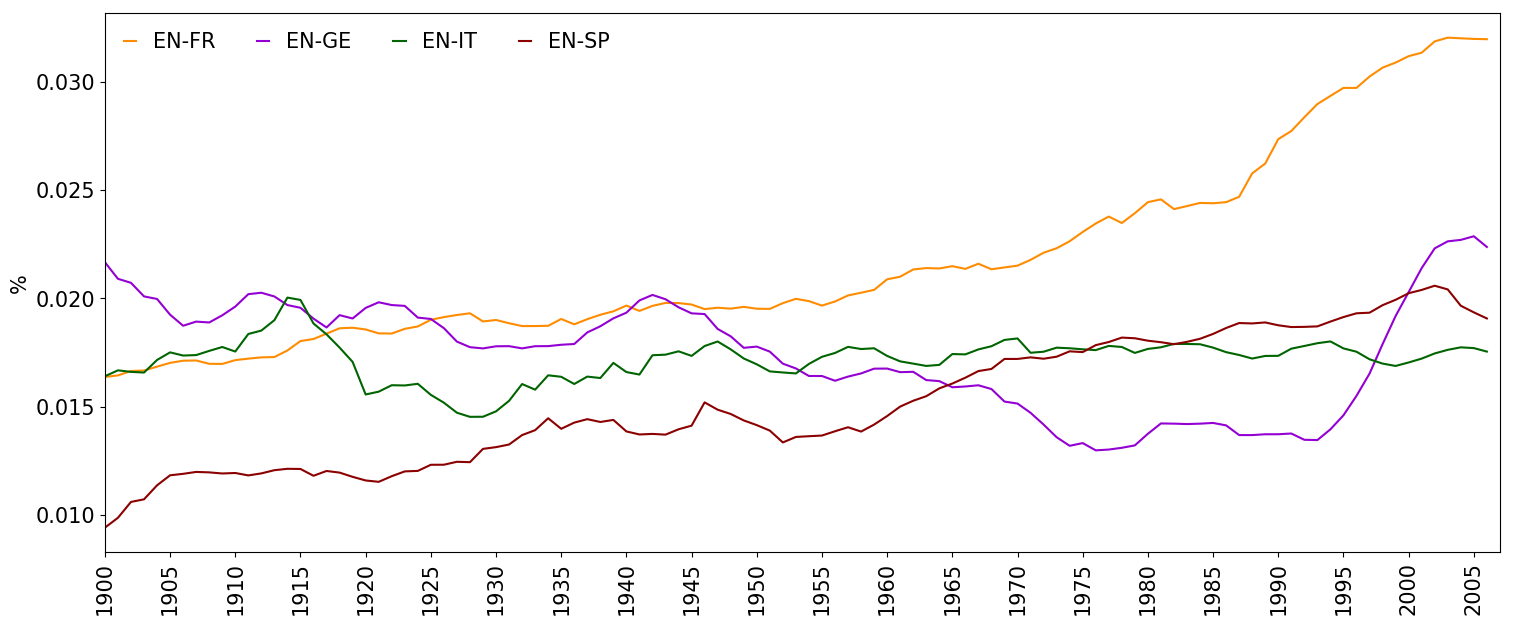
\includegraphics[width=14.5cm, height=7cm]{Cap_4/PF1_S2_EN.png}
				\label{fig.ST_a_EN}}
		\end{subfigure}
		
		\vspace{0.4cm}
		
		\begin{subfigure}
			[Los demás en el inglés.]{
				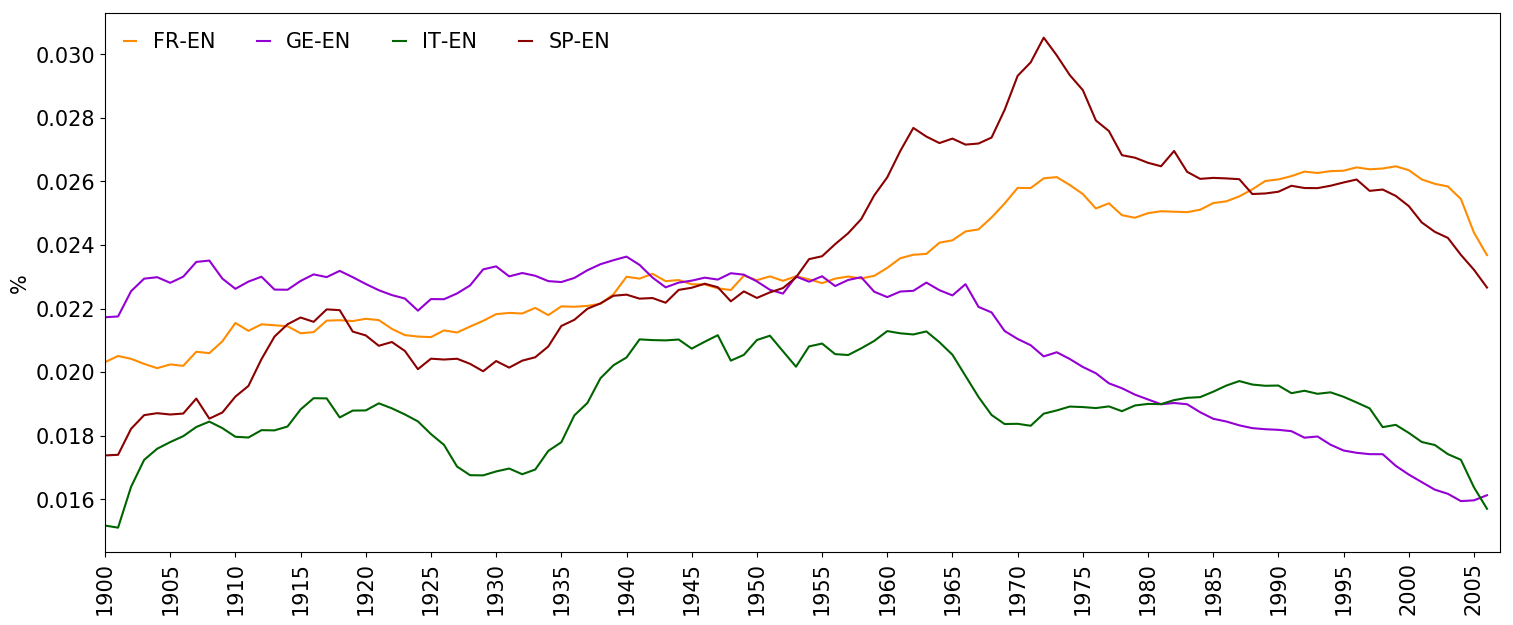
\includegraphics[width=14.5cm, height=7cm]{Cap_4/PF2_S2_EN.png}
				\label{fig.ST_b_EN}}
		\end{subfigure}
		
		\caption{Uso para el inglés}
		\label{fig.ST_EN}
	\end{center}
\end{figure}


Analizando la primera figura, el uso del ingles en los demás ha visto un continuo incremento posterior a 1945 en el francés, el italiano y el español, mientras que en el alemán se da posterior a 1990, año de la finalización del socialismo en Europa con la re-unificación de Alemania, además tras la re-unificación Alemania crece como potencia. 

Del conjunto de prestamos acumulados posteriores a 1945 en los cuatro receptores, el significado común de las palabras son términos políticos, económicos y referentes a la industria como  \textit{capital}, \textit{dollar}, \textit{invesment}, \textit{relations}, \textit{institutions}, \textit{internet} y \textit{software}. El campo semántico de estas palabras, confirma lo encontrado en los prestamos nuevos,  el inglés se ha beneficiado de estas áreas para ser exportado, utilizado y ser el idioma común para transmitir información. 


En los últimos cincuenta años, los idiomas mas comunes en el ingles han sido el español y el francés,  su crecimiento se propaga a partir de  1950, año posterior a la guerra, donde Alemania e Italia fueron derrotados por países de habla inglesa, siendo este un factor que haga decaer al alemán e italiano. El mayor pico  caracterizado por el español,  se relaciona con Aspectos como la proximidad geográfica entre Estados Unidos con Latinoamérica,  el aumento de las migraciones de personas entre ambos costados (siendo mayor el flujo hacia Estados Unidos) surgen como posibilidades del incremento.


\newpage
\subsection{Francés}

\begin{figure}[h!]
	\begin{center}
		\begin{subfigure}
			[El francés en los demás.]{
				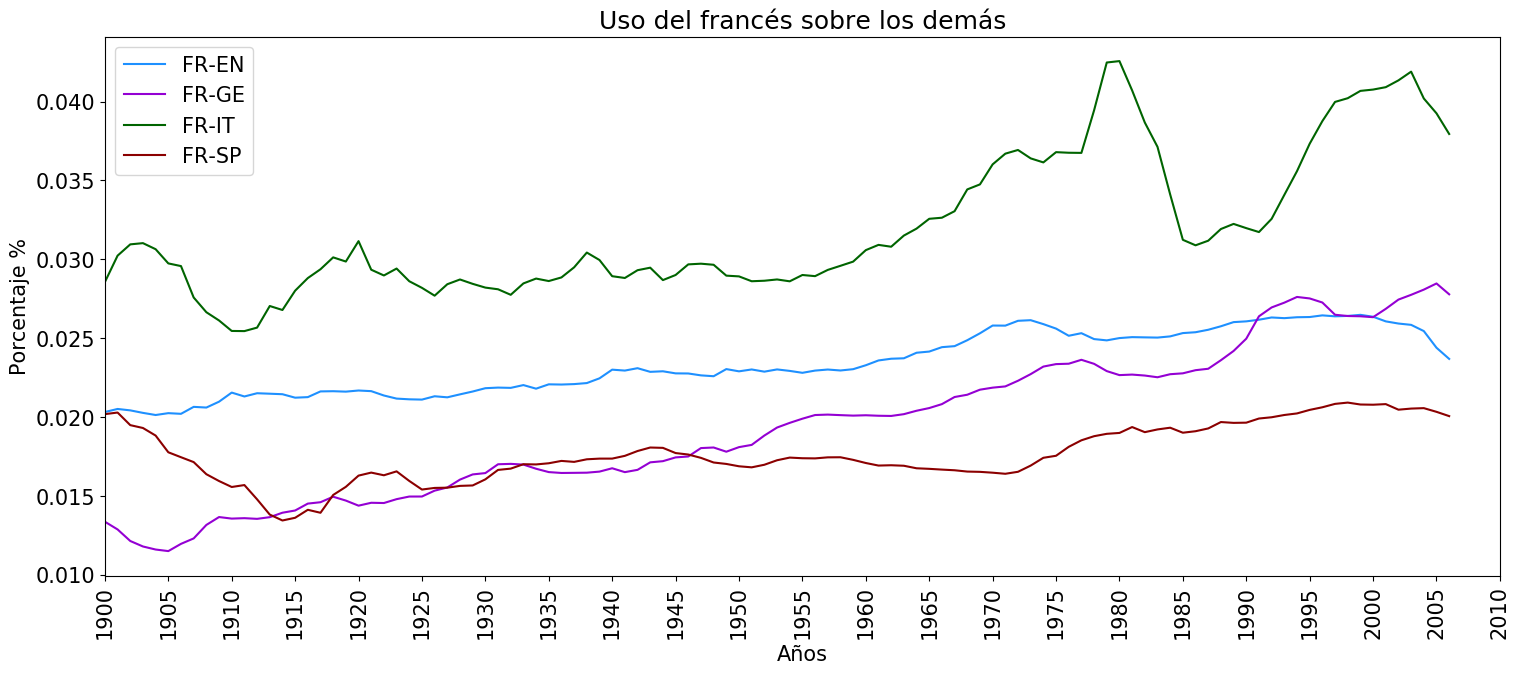
\includegraphics[width=14.5cm, height=7cm]{Cap_4/PF1_S2_FR.png}
				\label{fig.ST_a_FR}}
		\end{subfigure}
		
		\vspace{0.4cm}
		
		\begin{subfigure}
			[Los demás en el francés.]{
				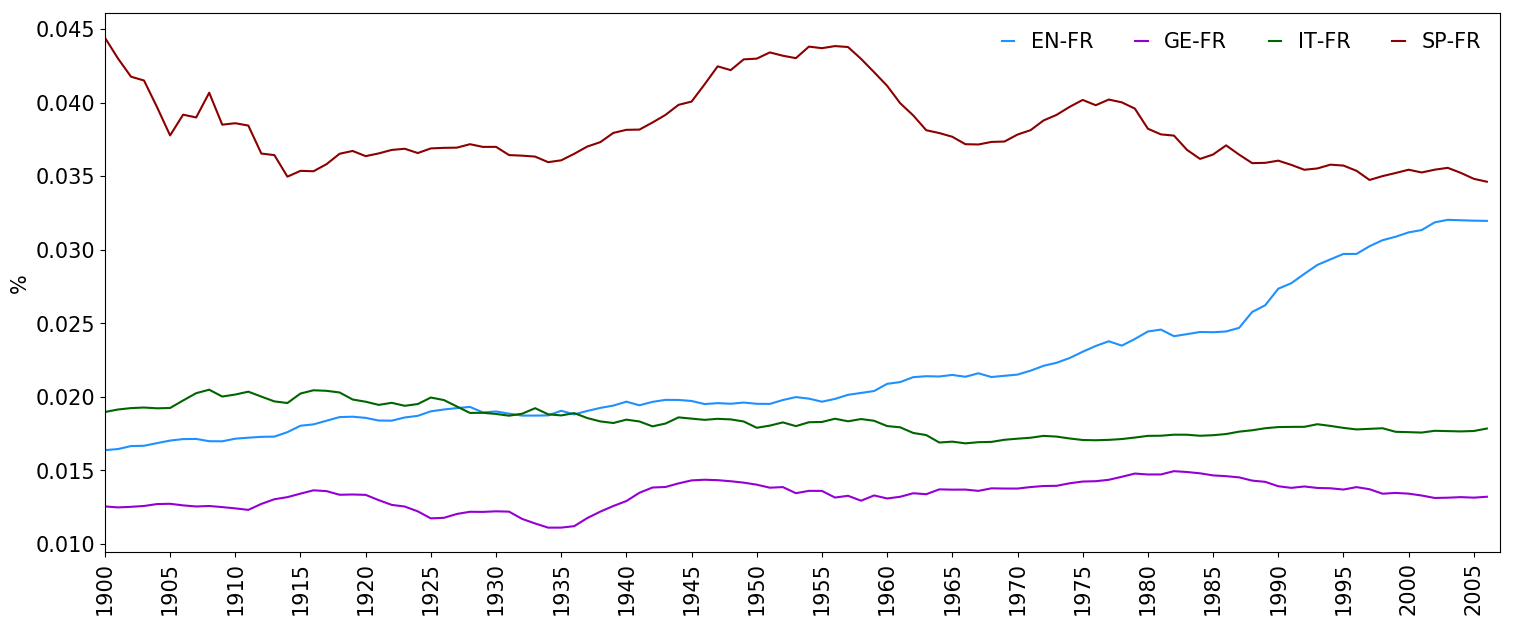
\includegraphics[width=14.5cm, height=7cm]{Cap_4/PF2_S2_FR.png}
				\label{fig.ST_b_FR}}
		\end{subfigure}
		
		\caption{Uso para el francés.}
		\label{fig.ST_FR}
	\end{center}
\end{figure}


A pesar de que el idioma que más préstamos toma del francés es el inglés,  el idioma que más utiliza el francés ha sido el italiano,  aspecto que se mantuvo durante todo el siglo del análisis.  Recapitulando lo comentado en los análisis de los préstamos,  el peso que tuvo la segunda guerra fue un detonante para que el uso entre los idiomas cambiase durante y posterior al conflicto,  en el caso del alemán y del inglés,  el empleo del francés en ellos aumentó tras finalizar el conflicto.  A pesar de que el español y el francés provienen de la familia de las lenguas romances,  el uso del francés en el español se ha mantenido sin mayores alteraciones.



El caso de cómo son utilizados los demás idiomas en el francés,  hay un dominio de las palabras con origen español, seguido por las de origen inglés; aunque el español ha sido el más empleado en el francés,  el inglés a partir de 1940 comienza a ser más frecuentado,  recortando en cada año la diferencia con el español,  siendo en la última parte del estudio  menor al 0.05$\%$, incluso si la base de datos abarcara más años posteriores al 2009, es probable que el uso el inglés pase al español. 



\newpage
\subsection{Alemán}

\begin{figure}[h!]
	\begin{center}
		\begin{subfigure}
			[El alemán en los demás.]{
				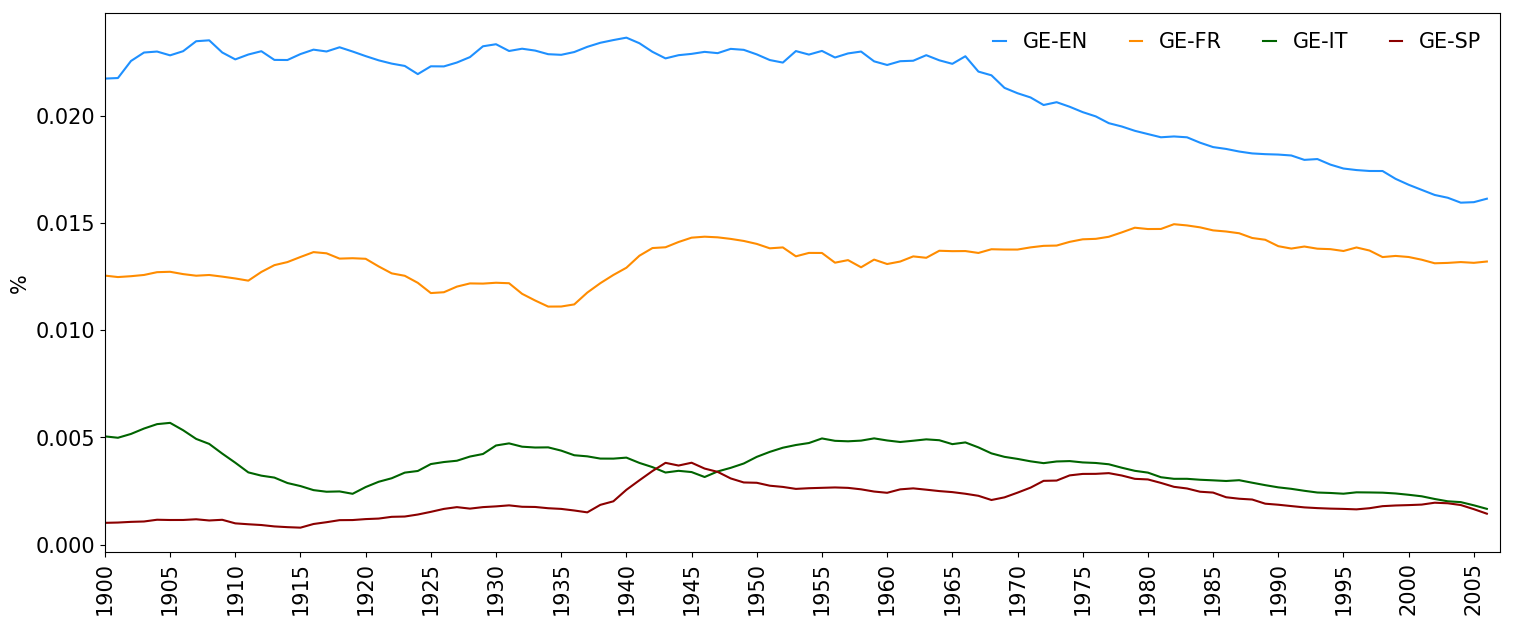
\includegraphics[width=14.5cm, height=7cm]{Cap_4/PF1_S2_GE.png}
				\label{fig.ST_a_GE}}
		\end{subfigure}
		
		\vspace{0.5cm}
		
		\begin{subfigure}
			[Los demás en el alemán.]{
				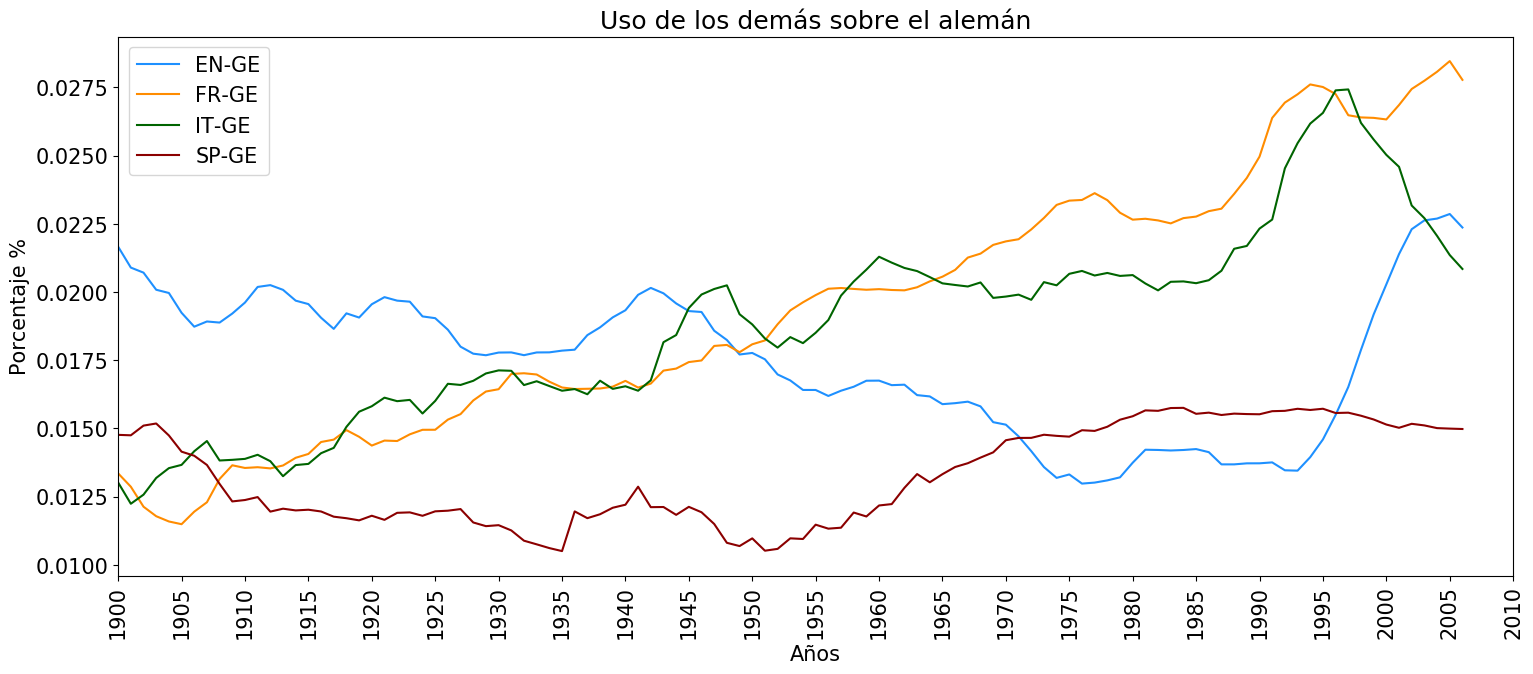
\includegraphics[width=14.5cm, height=7cm]{Cap_4/PF2_S2_GE.png}
				\label{fig.ST_b_GE}}
		\end{subfigure}
		
		\caption{Uso para el alemán.}
		\label{fig.ST_GE}
	\end{center}
\end{figure}



De acuerdo a la tabla \ref{table.PA},  el inglés, el francés, el italiano y el español, son en ese orden idiomas que más préstamos tienen provenientes del alemán, a pesar de que el alemán sea en cada uno el idioma del que menos se componen.  El orden de los idiomas que más emplean el alemán es el mismo que los idiomas que más se componen del alemán, siendo el único caso donde la mayor cantidad es también el mayor uso. Una razón de esta característica es que tanto el alemán como el inglés provienen de la misma familia lingüística, la germánica,  siendo más comunes las palabras entre ellos  que con las lenguas romances.

El sentido de cómo se utilizan los demás idiomas en el alemán, no presenta la característica anterior,   donde se ha alternado entre el inglés, el francés y el italiano el idioma que es más utilizado en el alemán.  El inglés fue el más empleado en la primera mitad del siglo, mientras que posterior a la guerra que ha sido el común detonante para que se altere el uso de un idioma en otro,  francés e italiano rolaron el papel del idioma más común en el alemán. 


\newpage
\subsection{Italiano}

\begin{figure}[h!]
	\begin{center}
		\begin{subfigure}
			[El italiano en los demás.]{
				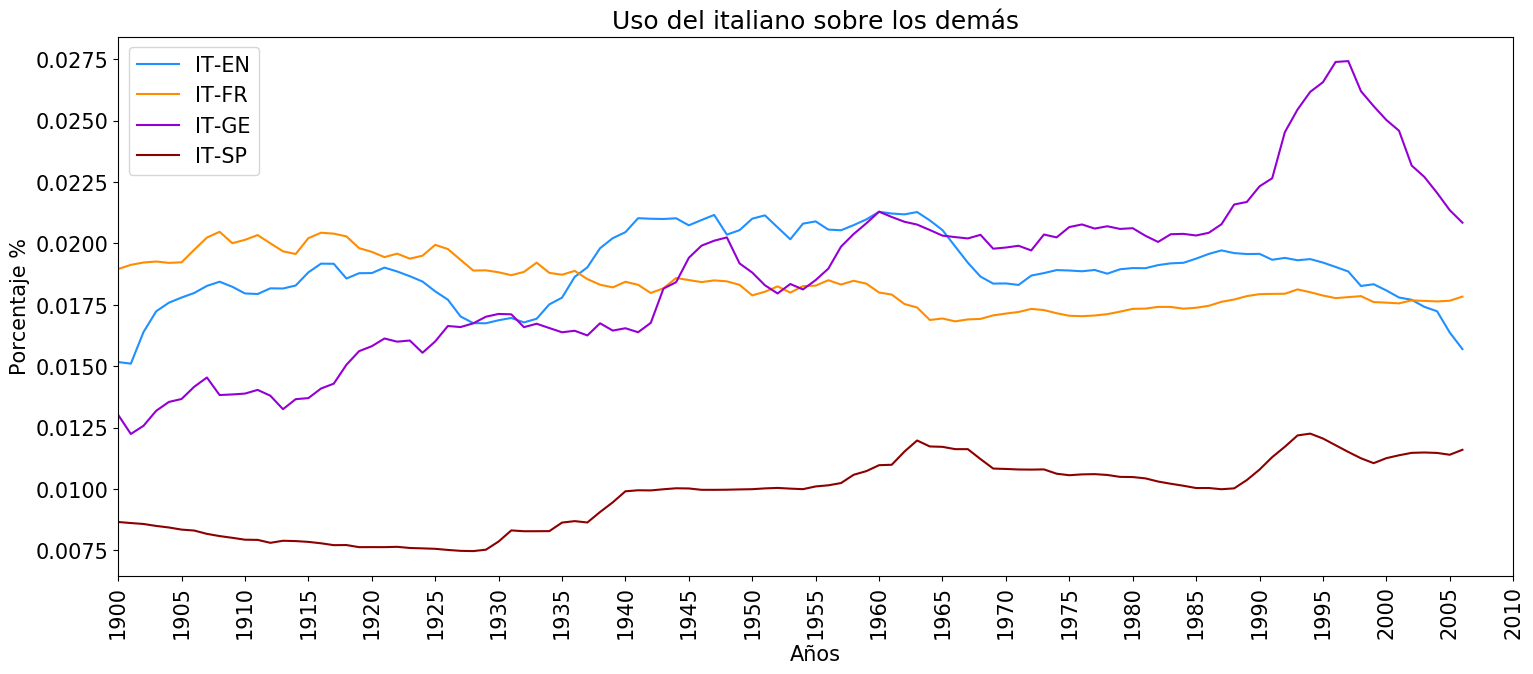
\includegraphics[width=14.5cm, height=7cm]{Cap_4/PF1_S2_IT.png}
				\label{fig.ST_a_IT}}
		\end{subfigure}
		
		\vspace{0.5cm}
		
		\begin{subfigure}
			[Los demás en el italiano.]{
				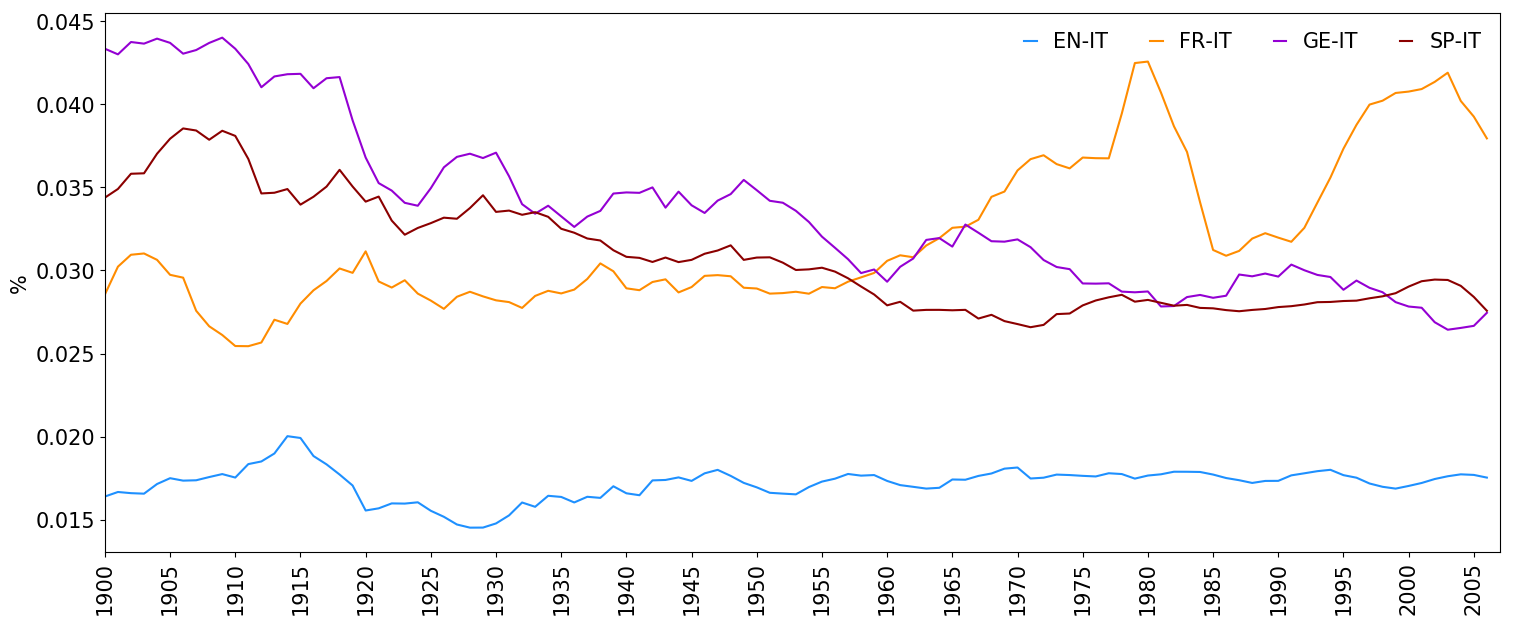
\includegraphics[width=14.5cm, height=7cm]{Cap_4/PF2_S2_IT.png}
				\label{fig.ST_b_IT}}
		\end{subfigure}
		
		\caption{Uso para el italiano.}
		\label{fig.ST_IT}
	\end{center}
\end{figure}

Los idiomas en los que el italiano ha tenido una mayor influencia han sido el inglés, el francés y el alemán pese a que el español es el idioma que más préstamos contiene del  italiano,  circunstancias como la cercanía geográfica entre los países de habla alemán con Italia alude al  mayor uso del italiano en este idioma a partir de  la segunda mitad del siglo,  respecto al inglés,  la intervención de personajes  italianos en la historia y el hecho de que el inglés se compone de palabras de origen grecolatino,  permite que el italiano sea una lengua fuerte en el inglés;  las afirmaciones anteriores se han respaldado en que las palabras de contenido han sido previamente relacionadas  a sucesos donde han intervenido estos países.


La forma de actuar de los demás idiomas en el italiano no es recíproca a la forma en que el italiano interviene en ellos.  El caso del inglés es particular, porque a pesar del impacto que ha manifestado el inglés en los demás idiomas  en los últimos cincuenta años por la globalización,  en el italiano ha sido el único idioma donde no ha sido dominante en algún punto, o donde no ha crecido más que los demás.  El alemán ha sido más importante al comienzo del siglo y decae tras finalizar la segunda guerra mundial, para imponerse el francés como el idioma que más es utilizado en el italiano. 


\newpage
\subsection{Español}

\begin{figure}[h!]
	\begin{center}
		\begin{subfigure}
			[El español en los demás.]{
				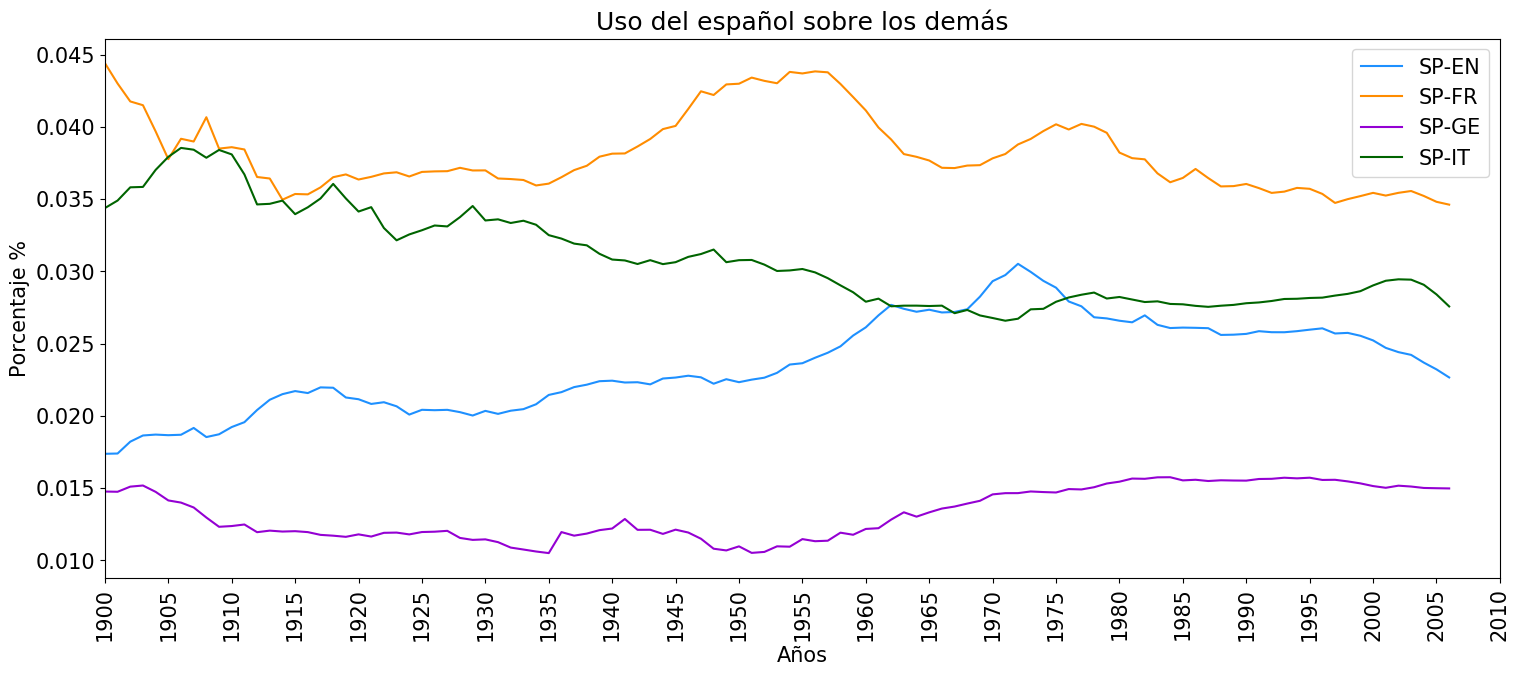
\includegraphics[width=14.5cm, height=7cm]{Cap_4/PF1_S2_SP.png}
				\label{fig.ST_a_SP}}
		\end{subfigure}
		
		\vspace{0.5cm}
		
		\begin{subfigure}
			[Los demás en el español.]{
				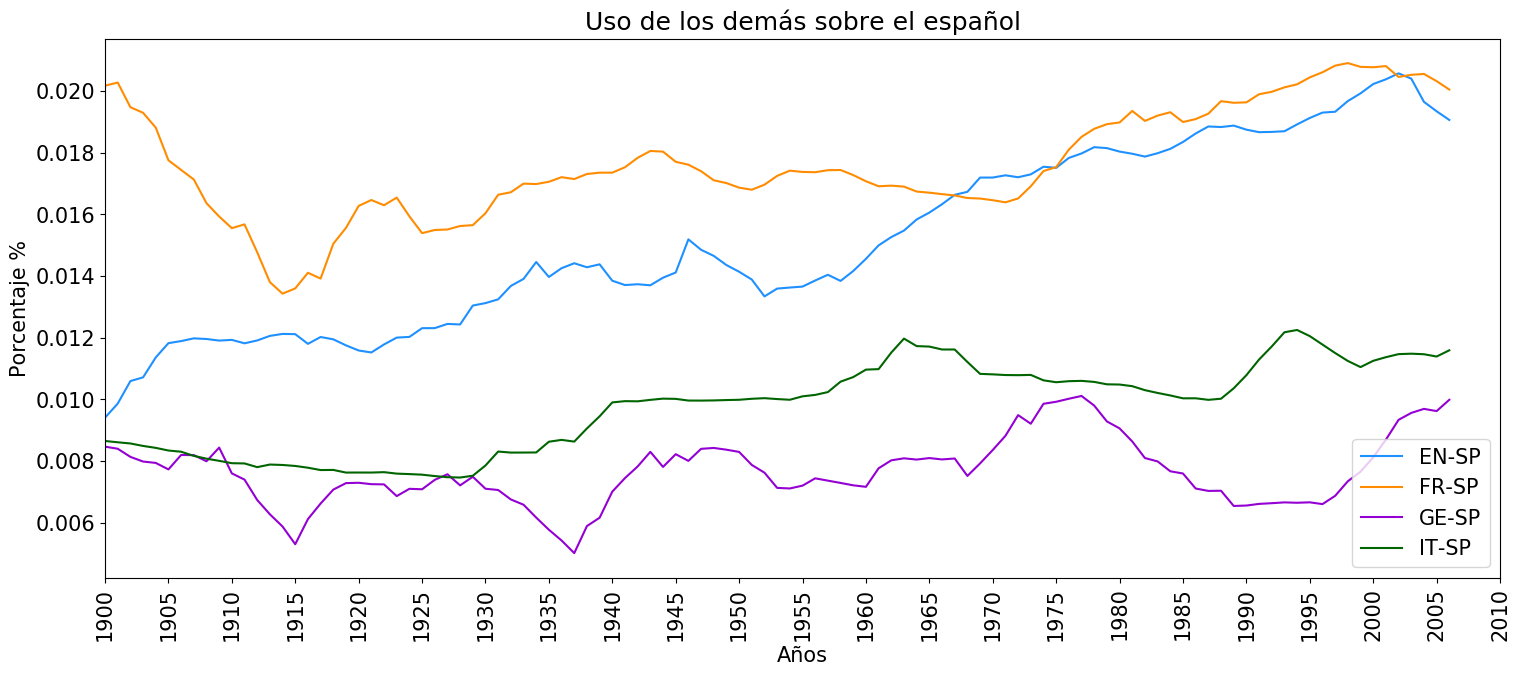
\includegraphics[width=14.5cm, height=7cm]{Cap_4/PF2_S2_SP.png}
				\label{fig.ST_b_SP}}
		\end{subfigure}
		
		\caption{Uso para el español.}
		\label{fig.ST_SP}
	\end{center}
\end{figure}


Entre los gráficos del apendice 1 de uso entre un determinado idioma y el español, se observó que el español ha sido más influyente en los demás que los demás en él,  siendo el francés el idioma donde el español es más utilizado, a pesar de que la cantidad de préstamos en el italiano es mayor, la causa mas lógica  de esta situación es el provenir ambos de la familia de las lenguas romances. 

Entre la forma en la que se usan los préstamos de los demás idiomas en el español,  en los últimos cincuenta años, la mayor influencia se ve compartida entre las palabras que vienen del francés y  del inglés;  la familia de las lenguas romances y sus similitudes hacen posible que el francés tome relevancia, mientras que la globalización y el crecimiento económico de países de habla inglesa hace relevante al inglés en el español.   Por otro lado,  el italiano y el alemán  no presentan el mismo crecimiento que el francés y el inglés,  por parte del italiano se ha comentado que al ser lengua romance al igual que el español,  el periodo donde los préstamos modificaban el uso del idioma receptor pudiese ser tan antiguo como el surgimiento de los idiomas,  por ello comparten gran cantidad de palabras pero estas no alteran el comportamiento del receptor; mientras que en el caso del alemán la poca relación con el español y el no haber existido un evento que los involucren,  hace que estos idiomas no se hayan mezclado como los demás,  por ejemplo alrededor de 1915 y 1935,  el alemán en el español es casi nulo, a pesar de que en esas fechas se desarrollaron las grandes guerras.


\newpage
\section{Comentarios del método}

